\chapter{Implémentation du système}
\chaptermark{Système}
\minitoc
\newpage

\section{Introduction}

Le système de recommandation suivant est construit sur des données récoltées à travers le scraping des sites des fournisseurs de jungle Bike. Après cette étape les données ont subi des séries de nettoyages afin d’avoir la structure idéale pour la construction des modèles de machine learning. Les principaux outils qui interviendront dans la mise place de ce système seront Tensor Flow, Keras et Pytorch. Dans les lignes qui suivront nous allons faire l’exploration de la donnée afin d’avoir des informations statistiques sur les données. Par la suite nous allons appliquer des modèles de deep learning analyser leur performance et choisir le meilleur modèle pour notre jeu de données.

\newpage
\section{Analyse de données}
\subsection{Aperçu du jeu de donnée:}
\begin{figure}[h]
\begin{center}
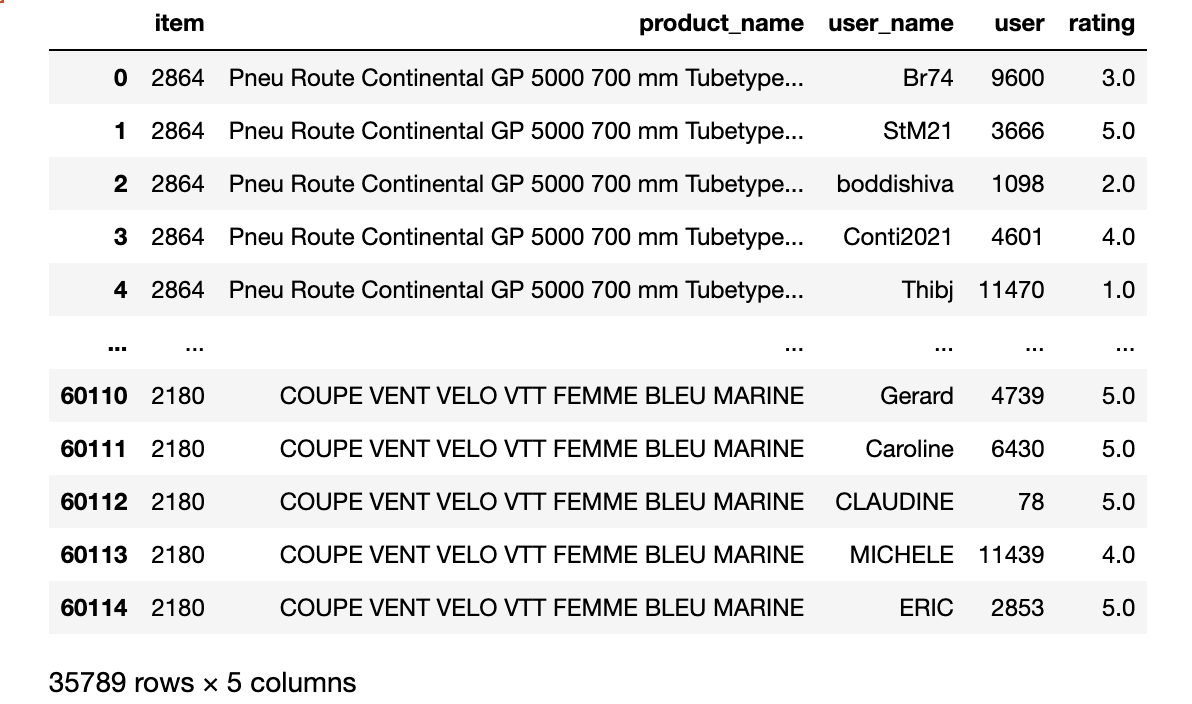
\includegraphics[width=15cm,height=10cm]{images/model_dataset.png}
\caption[Informations sur le produit le client et son vote]{Informations sur le produit le client et son vote}
\label{monlabel}
\end{center}
\end{figure}
\newpage

\subsection{Statistiques sur la dataset:}
\begin{figure}[h]
\begin{center}
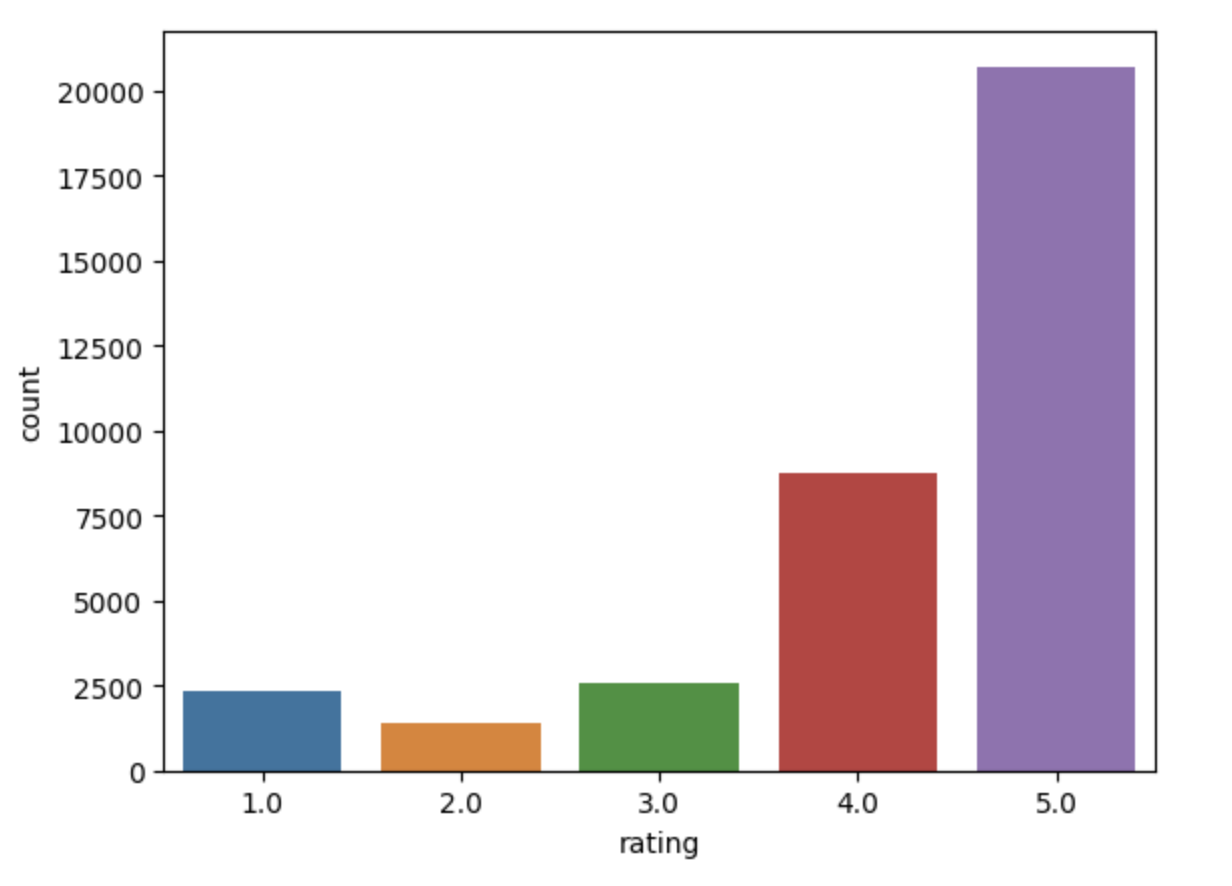
\includegraphics[width=15cm,height=10cm]{images/user_proportion.png}
\caption[Nombre de produit voté en fonction du score]{Nombre de produit voté en fonction du score}
\label{monlabel}
\end{center}
\end{figure}

\begin{figure}[h]
\begin{center}
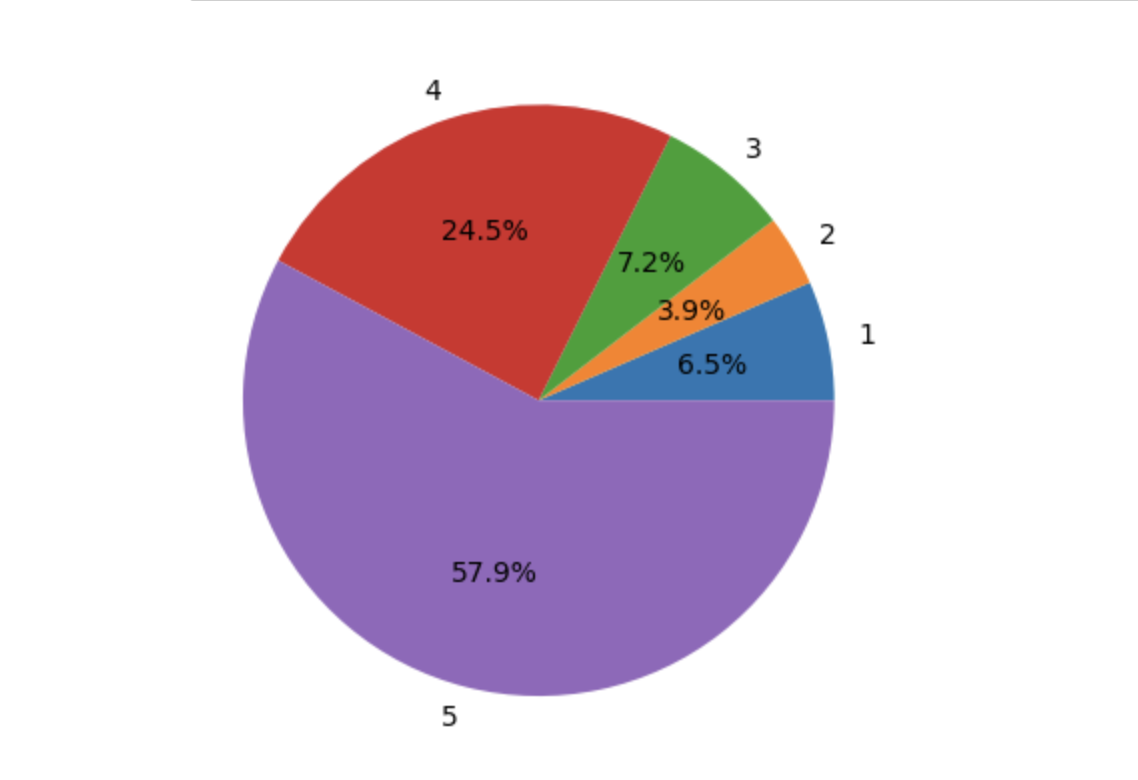
\includegraphics[width=15cm,height=10cm]{images/pie_user_vote.png}
\caption[Proportion du nombre de produit voté en fonction du score]{Proportion du nombre de produit voté en fonction du score}
\label{monlabel}
\end{center}
\end{figure}
\newpage

\subsection{Meilleurs produits et Clients par rapport aux votes:}
\begin{figure}[h]
\begin{center}
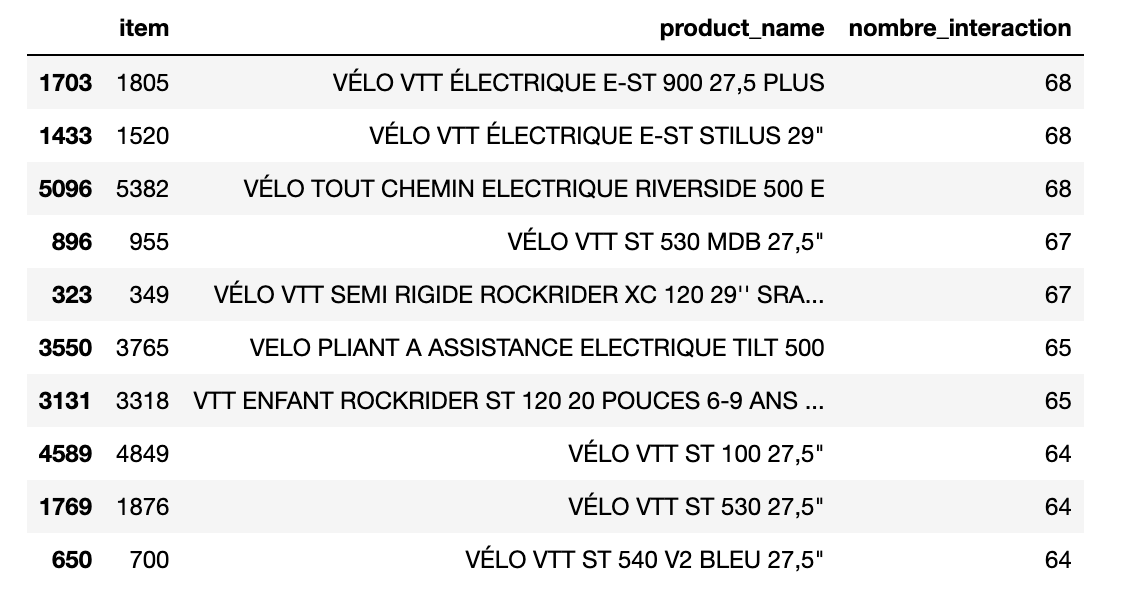
\includegraphics[width=15cm,height=8cm]{images/top_10_products.png}
\caption[Top 10 des meilleurs produits avec plus de la moitié des votes supérieurs au score 3]{Top 10 des meilleurs produits avec plus de la moitié des votes supérieurs au score 3}
\label{monlabel}
\end{center}
\end{figure}

\begin{figure}[h]
\begin{center}
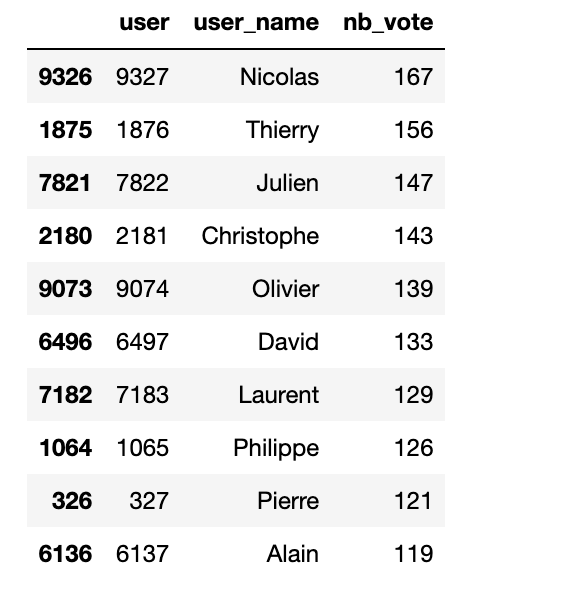
\includegraphics[width=10cm,height=8cm]{images/top10_users.png}
\caption[Top 10 des Meilleurs clients]{Top 10 des Meilleurs clients}
\label{monlabel}
\end{center}
\end{figure}


\clearpage



\section{Application des différents modèles au jeu de données}
\subsection{Matrice de Factorisation:}
Tout d’abord on fait passer chacun des vecteurs d’item et user dans une couche d’\textbf{Embedding},
Ensuite un produit matriciel est effectué entre le vecteur d’item et de user transformé.
Le produit résultant est directement passé au modèle et compilé avec un optimiseur \textbf{Adam} avec les métriques \textbf{MAE} et \textbf{MSE}.

\subsection{Combinaison Matrice de Factorisation et Réseau de Neurone:}
On fait passer chacun des vecteurs d’item et user dans une couche d’\textbf{Embedding},
Ensuite un produit matriciel est effectué entre le vecteur d’item et de user transformé.
Le produit résultant est passé à deux couches \textbf{Dense} pour ensuite produire une sortie qui sera passée au modèle.
Cette dernière est compilée  avec un optimiseur \textbf{Adam (learning rate de 0.1)} avec les métriques \textbf{MAE} et \textbf{MSE}.

\subsection{Combinaison Matrice de Factorisation et Multilayer perceptron:}
On fait passer chacun des vecteurs d’item et user dans une couche d’\textbf{Embedding},
Ensuite on concatène les vecteurs d’item et de user transformé.
Le résultat est passé aux couches \textbf{Dense, BatchNormalization, Dense, BatchNormalization},  pour ensuite produire une sortie du multiplayer perceptron.
On reprend les vecteurs d’entrée passés en dans les couches d’\textbf{Embedding} qui vont subir un produit matriciel. Cette dernière est combinée à la sortie du perceptron multicouche précédent pour passer dans la couche \textbf{Dense}. La sortie résultante passe dans le modèle et compilé avec un optimiseur \textbf{Adam (learning rate de 0.01)} avec les métriques \textbf{MAE} et \textbf{MSE}.

\subsection{LSTM: Long Short Term Memory}
Pour ce modèle on transforme le jeu de donnée pour avoir chaque user avec les produits interagit et le son score sous la forme:
\begin{figure}[h]
\begin{center}
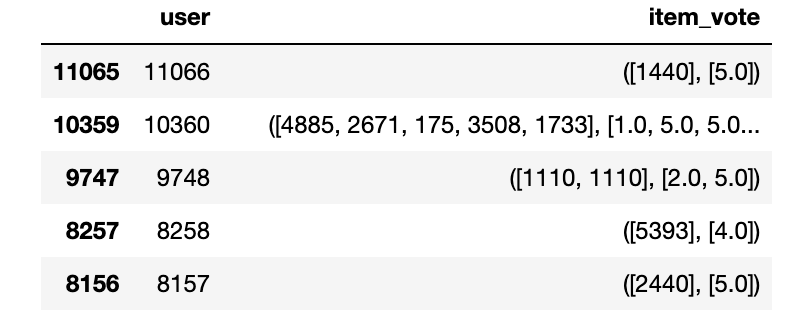
\includegraphics[width=10cm,height=4cm]{images/lstm_data.png}
\caption[Utilisateurs avec leurs interactions avec les produits]{Utilisateurs avec leurs interactions avec les produits}
\label{monlabel}
\end{center}
\end{figure}
Le modèle est formé d’une couche d’Embedding avant de passer dans la couche de \textbf{LSTM}.
Une couche \textbf{Linéaire} est appliquée à la sortie pour produire la sortie définitive.
La métrique d’évaluations \textbf{Mean Squared Error} est appliquée pour les étapes d’apprentissage et de test.

\clearpage
\section{Tests et validation: Analyse des RMSE des différents modèles}
\subsection{Statistiques de performance des modèles}
\begin{figure}[!htb]
\begin{center}
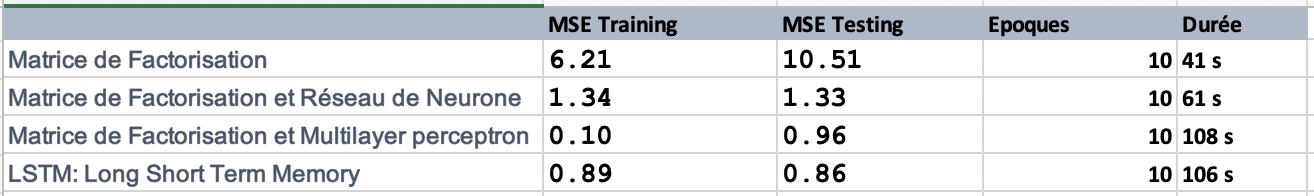
\includegraphics[width=16cm,height=3cm]{images/validation_statistics.png}
\caption[Statistiques de performanes des modèles]{Statistiques de performanes des modèles }
\label{monlabel}
\end{center}
\end{figure}
\subsection{Evolution d'apprentissage des modèles en fonction du nombre d'époque}
\begin{figure}[!htb]
\begin{center}
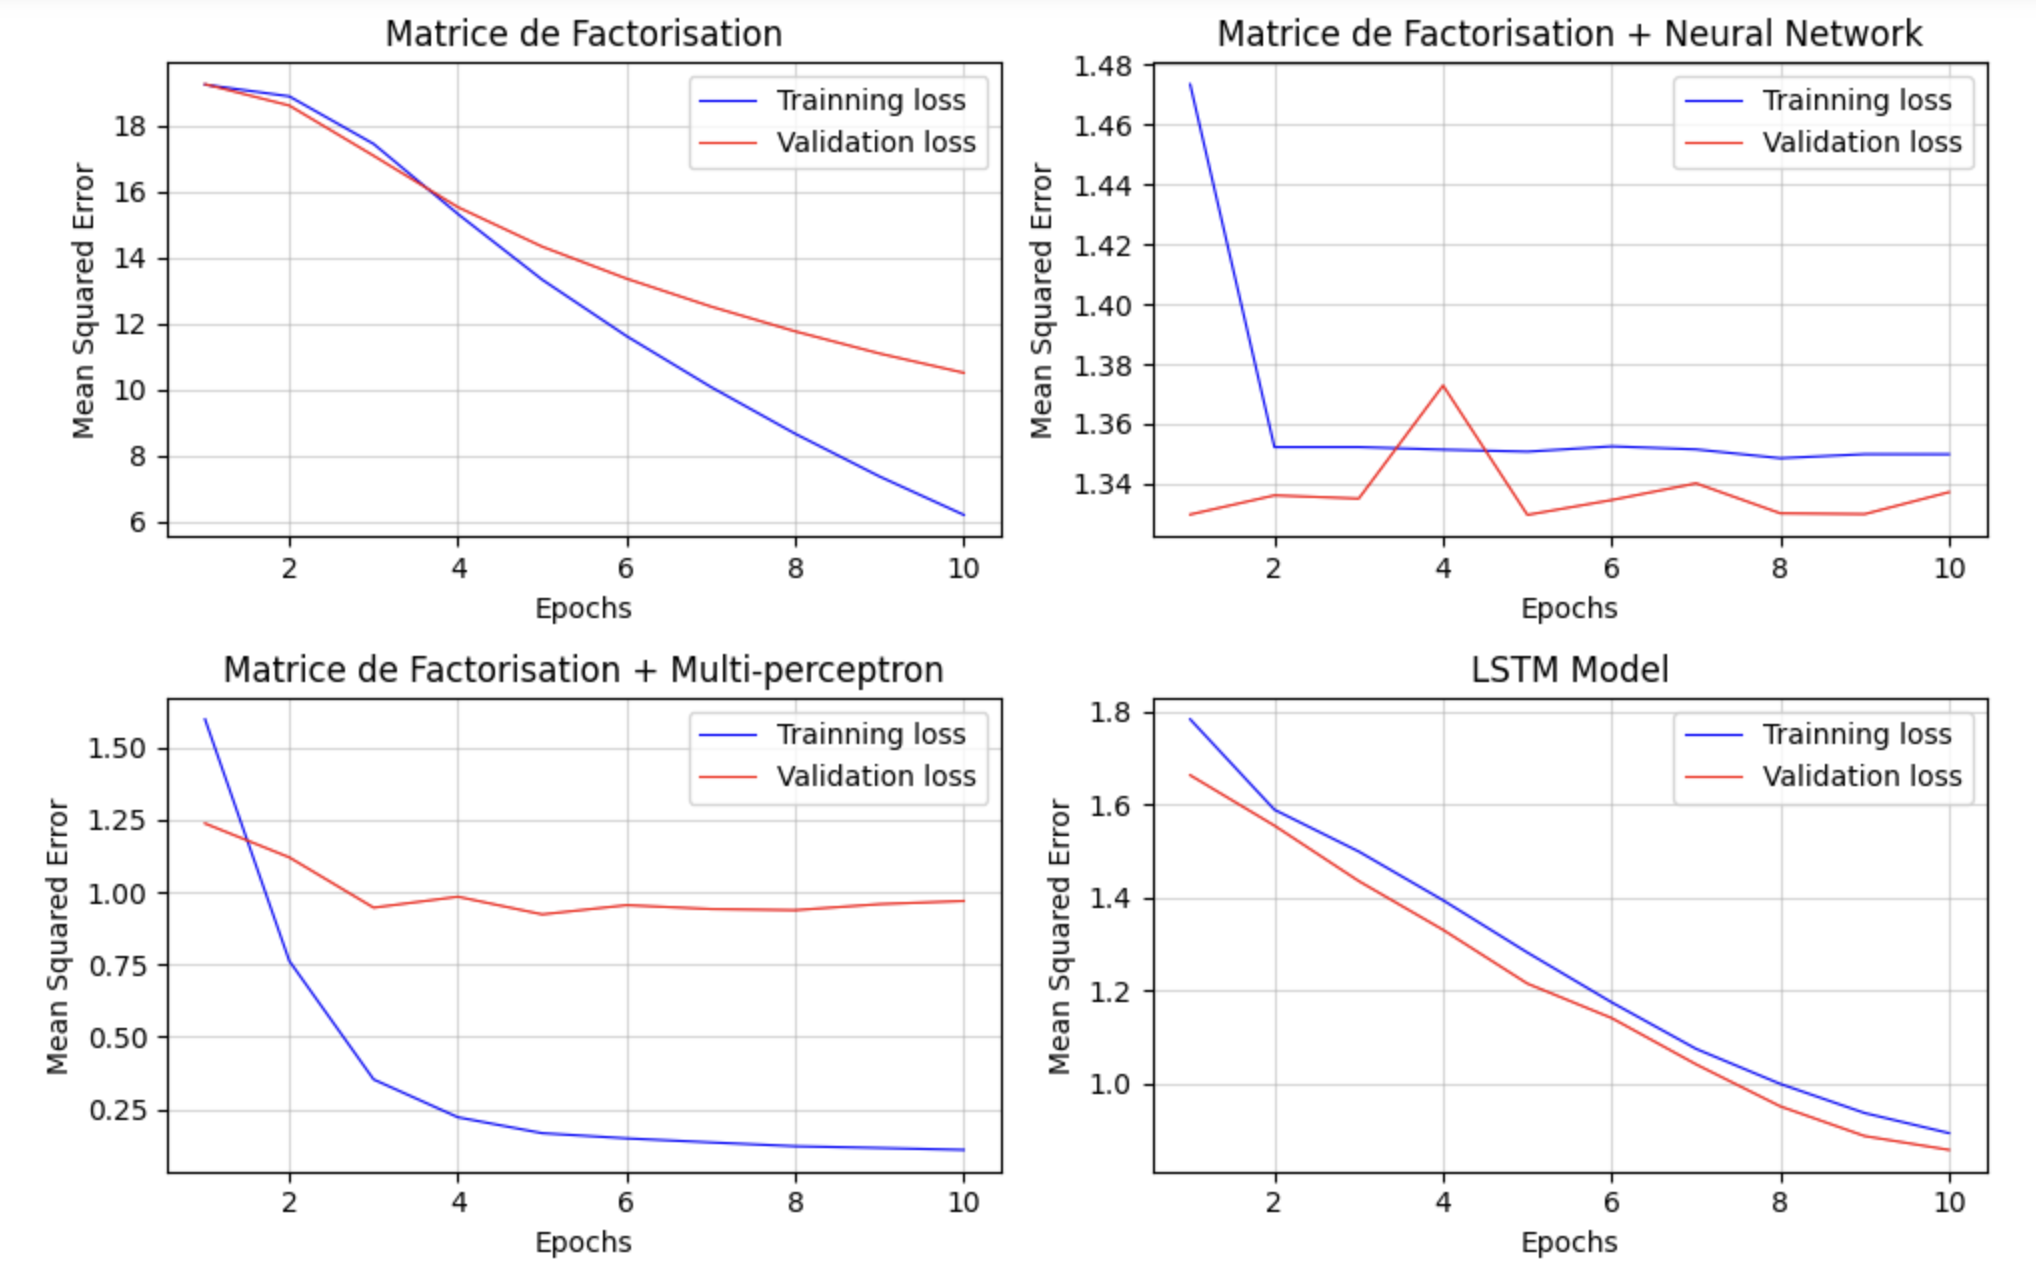
\includegraphics[width=16cm,height=16cm]{images/model_evaluation.png}
\caption[Etude de la validation des modèles]{Etude de la validation des modèles}
\label{monlabel}
\end{center}
\end{figure}

\clearpage
\section{Conclusion}
D'après les résultats, on remarque tout d’abord que la matrice de factorisation seule est le modèle le moins performant avec plus d'erreurs. En associant le modèle de matrice de factorisation avec les réseaux de neurones on remarque des améliorations sur les résultats malgré que le temps d’apprentissage augmente. En prenant en compte la courbe de perte d’erreur nous pouvons remarquer que le modèle issu de la combinaison de la matrice de factorisation avec les perceptron multicouche ont enregistré moins d'erreurs à l’apprentissage.